\chapter{Aplicación sigue personas}
\label{cap:capitulo5}
Ahora que ya está integrado ROS2 dentro de la plataforma de VisualCircuit, se han creado varios proyectos usando los bloques drivers.
El primero de ellos será un comportamiento de \textit{follow-person} usando reconocimiento visual.

\section{Descripción del comportamiento y escenario}
\label{sec:FP_intro}

El comportamiento sigue-personas o \textit{follow-person} que buscamos desarrollar consiste en rotar en el sitio hasta encontrar
a una persona mediante algoritmos de detección visual de objetos y mantener a la persona centrada en la imagen, a la vez que se
mantiene al robot a una distancia constante de la persona. Este comportamiento se ha dividido en dos etapas: seguimiento estático
(sólo velocidad angular) y seguimiento completo (velocidad angular y lineal).\\

Para esta aplicación se ha usado el robot TurtleBot2 (\ref{sec:turtlebot2}). Dado que sólo se necesita la visión para seguir a la
persona, sólo se usa la cámara RGB-D como sensor, ya que también ofrece la profundidad leída en cada \textit{pixel} y sirve para
mantener al robot a una distancia constante de la persona.

Para el entorno de pruebas se ha usado un modelo de persona teleoperada (figura \ref{fig:teleop_person}) que creó en su TFG Carlos
Caminero\footnote{\url{https://github.com/RoboticsLabURJC/2021-tfg-carlos-caminero/tree/main/amazon_hospital/hospital_world}}, compañero
de la carrera.

\begin{figure} [H]
    \begin{center}
        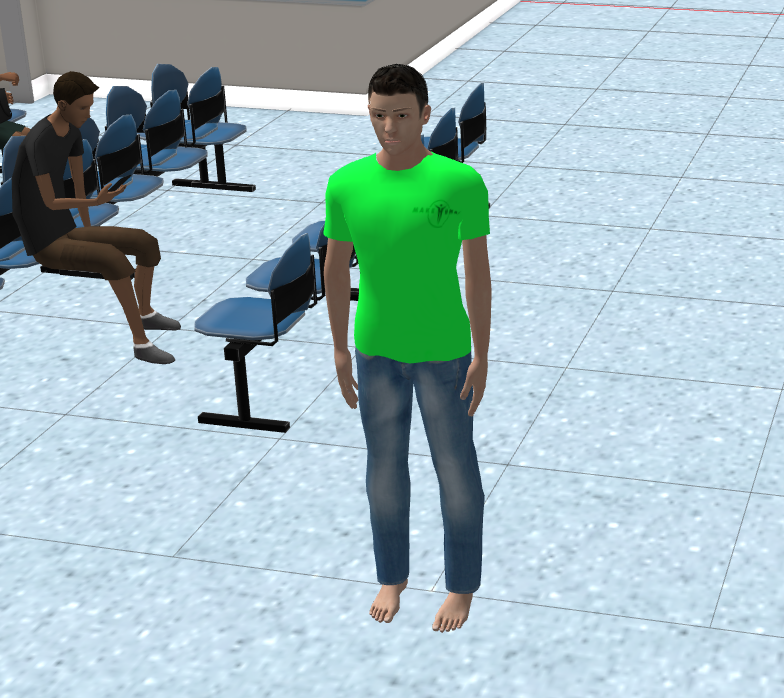
\includegraphics[width=6cm]{figs/c5/elman.png}
    \end{center}
    \caption[Modelo de persona en gazebo]{Modelo de persona teleoperable en gazebo.}
    \label{fig:teleop_person}
\end{figure}
El mundo que usó Carlos incluía muchos elementos del entorno que no son necesarios en este caso, por lo que se ha modificado el
mundo para dejar únicamente al robot y a la persona. El modelo del robot usado en las pruebas simuladas es el que se mencionó en el
capítulo \ref{subsec:turtlebot2_sim}.\\

Las pruebas realizadas con el robot TurtleBot2 real se han hecho en el laboratorio docente de robótica, mencionado en la sección \ref{subsec:urjc},
instalando en el robot la cámara como único sensor (sección \ref{subsec:asus_xtion}) y usando los motores de la base \textit{kobuki}
(sección \ref{subsec:turtlebot2_base}) como único actuador.

Para configurar correctamente los sensores del robot real se deben tener instalados los paquetes para
activar el kobuki (\ref{subsec:turtlebot2_base}), al igual que los necesarios para usar la cámara (\ref{subsec:asus_xtion}).
para conseguir que todo funcione correctamente se han usado los siguientes comandos:

\begin{code}[H]
    \begin{lstlisting}[language=bash]

$> ros2 launch asus_xtion asus_xtion.launch.py

$> ros2 launch ir_kobuki kobuki_rplidar.launch.py
    \end{lstlisting}
    \caption[Comandos para lanzar kobuki y cámara]{Comandos para activar la cámara con ROS2 y lanzar el kobuki con el láser.}
    \label{cod:coms_kobuki_laser_cam}
\end{code}

\section{Seguimiento de persona sólo con rotación}
\label{sec:FP1}

\subsection{Diseño del comportamiento}
\label{subsec:FP1_dis_comp}

En esta primera aproximación, buscaremos mantener a la persona centrada en la imagen usando únicamente movimiento angular.\\

La lógica que seguirá será la siguiente: recibir la imagen del \textit{topic} de la cámara y compartirla con el bloque de detección de objetos,
enviar la imagen con las detecciones al bloque \textit{screen} para visualizar en tiempo real lo que está analizando el robot,
mandando también los resultados a un bloque encargado de decidir el comportamiento que seguir. Este bloque activa un PID en caso
de que haya una persona en la imagen o el comportamiento de rotación en caso de que no se haya encontrado ninguna.
En ambos casos, se envía la decisión a los bloques que generan las velocidades y también al bloque \textit{MotorDriver} que se
ha desarrollado en la sección \ref{sec:motordriverros2}, que recibe tanto las distintas velocidades, como la decisión que se ha tomado, y
envía al \textit{topic} la que corresponda.

\begin{figure} [H]
    \begin{center}
        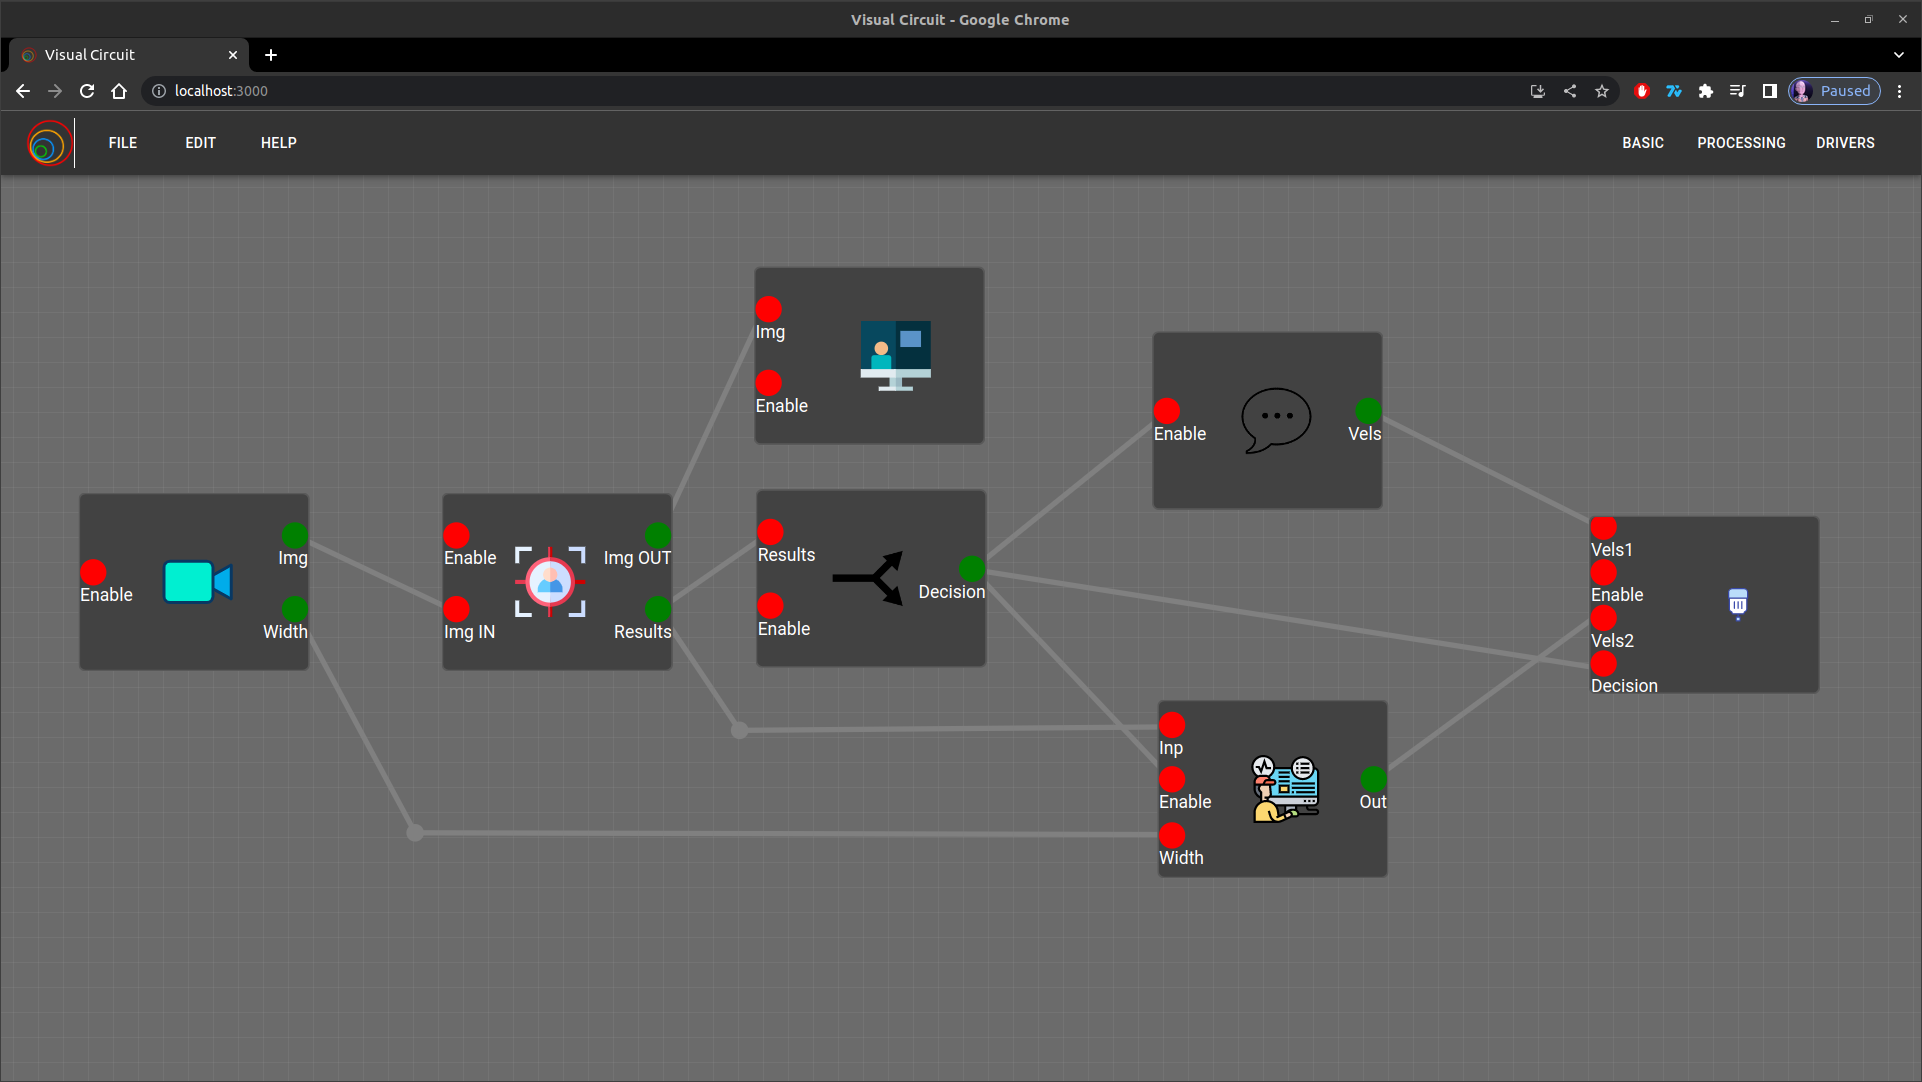
\includegraphics[width=10cm]{figs/c5/follow_person_initial.png}
    \end{center}
    \caption[Circuito sigue-personas inicial]{Circuito inicial del algoritmo sigue-persona.}
    \label{fig:initial_follow_person}
\end{figure}

\subsection{Bloques específicos de la lógica de esta aplicación}
\label{subsec:FP1_blocks}

El primer bloque de esta aplicación es el encargado de la detección de objetos mediante
yolov3\footnote{\textbf{YouOnlyLookOnce (YOLO)}: \url{https://pjreddie.com/darknet/yolo/}}, un algoritmo de detección de objetos a tiempo real que
permite identificarlos tanto en video como en imágenes usando redes neuronales (darknet\footnote{\textbf{DarkNet}: \url{https://pjreddie.com/darknet/}}).
El bloque ya está integrado en VisualCircuit, pero ha sido modificado para poder extraer también la localización de la
\textit{Bounding Box}\footnote{\textbf{Bounding Box}: Delimitación que se coloca alrededor de un objeto detectado por el algoritmo.}
que corresponde a la persona y compartirla con otros bloques.\\

Para ello, una vez obtenidos los nombres de los objetos encontrados, se recorre toda la lista comprobando si hay alguna persona,
en caso de haberla se envía la \textit{Bounding Box} correspondiente por el cable. En caso contrario se envía un \textit{array} con
cuatro valores ``-1'' para indicar que está vacío.

\begin{code}[H]
    \begin{lstlisting}[language=python]
        results = net.forward(outputNames)
        findObjects(results,frame)
        is_person = False
        for i in classIds:
            if(className[i] == "person"):
                is_person = True
                break
        to_send = [-1,-1,-1,-1]
        if(is_person):
            to__send = bbox[i]
        outputs.share_image("Img OUT", frame)
        outputs.share_array("Results", to__send)
    \end{lstlisting}
    \caption[Modificación al bloque detector de objetos]{Modificación al bloque de la detección de objetos.}
    \label{cod:mod_object_detector}
\end{code}

El siguiente bloque (\ref{cod:decision_follow_person}) es el que toma las decisiones de qué comportamiento seguir.
Para ello, primero se espera hasta recibir algún resultado de la visión y así no mover al robot antes de haber podido analizar la situación.
Una vez lleguen los resultados, se comprueba si es una \textit{Bounding Box} válida, en caso de serlo, la decisión será seguir lo que indique
el bloque PID para mantener a la persona centrada en la imagen.
En caso de ser una caja vacía (\textit{array} de ``-1'') se activa un contador para aplicar un filtro de paso bajo.
Este filtro permite evitar cambiar de comportamiento por pequeños errores en la detección de objetos.
Está establecido a 10, por lo que al llegar a 10 imágenes seguidas sin una persona en la imagen, se cambia de comportamiento al de la rotación
en su búsqueda.

\begin{code}[H]
    \begin{lstlisting}[language=python]
        def main(inputs, outputs, parameters, synchronise):
            auto_enable = True
            try:
                enable = inputs.read_number("Enable")
            except Exception:
                auto_enable = True
            while(True):
            # Wait for results
                results = inputs.read_array("Results")
                try:
                    if(results.any()):
                        break
                except Exception:
                    continue
    
            not_to_enable = 0
            to_enable = 1
            lowpass_filter = 10
            counter = 0
            while(auto_enable or inputs.read_number('Enable')):
                results = inputs.read_array("Results")
                if(results[0] != -1):
                    # Follow
                    counter = 0
                    outputs.share_number("Decision", 1)
                elif(counter < lowpass_filter):
                    # Follow but low-pass filter
                    counter += 1
                    outputs.share_number("Decision", 2)
                else:
                    # Rotation
                    outputs.share_number("Decision", 0)
    \end{lstlisting}
    \caption[Código bloque decisión sigue-persona]{Código del bloque de decisiones del sigue-persona.}
    \label{cod:decision_follow_person}
\end{code}

En cuanto al bloque que envía la velocidad correspondiente al comportamiento de rotación, tiene un bucle que lee la información que le llega
desde el cable y en caso de ser un "1" (\textit{True}) envia una velocidad angular de 1rad/s para el eje Z e informa en la terminal que el robot está rotando.

\begin{code}[H]
    \begin{lstlisting}[language=python]
    import numpy as np

    def main(inputs, outputs, parameters, synchronise):
        try:
            while 1:
                if(inputs.read_number('Enable')):
                    print("ROT")
                    vels = [0,0,0,0,0,1]
                    to_write = np.array(vels, dtype='<U64')
                    outputs.share_array("Vels", to_write)   
                    synchronise()
        except Exception as e:
            print("Error")
    \end{lstlisting}
    \caption[Código bloque rotación sigue-persona]{Código del bloque de la rotación del sigue-persona.}
    \label{cod:rotation_follow_person}
\end{code}

En casi de encontrar a una persona en la imagen, se activa el bloque PID\footnote{
    \textbf{PID}: Controlador proporciona, integral y derivativo.
        Mecanismo de control que, mediante sistema en lazo cerrado (realimentación), permite regular
        un valor (velocidad, temperatura, presión, etc)}.
Su estructura consiste en tres entradas (Resultados de la detección de objetos, ancho de la imagen y \textit{enable}), tres parámetros para las
tres constantes del controlador y una salida para la velocidad lineal y angular final que aplicaremos al robot.

\begin{figure} [H]
    \begin{center}
        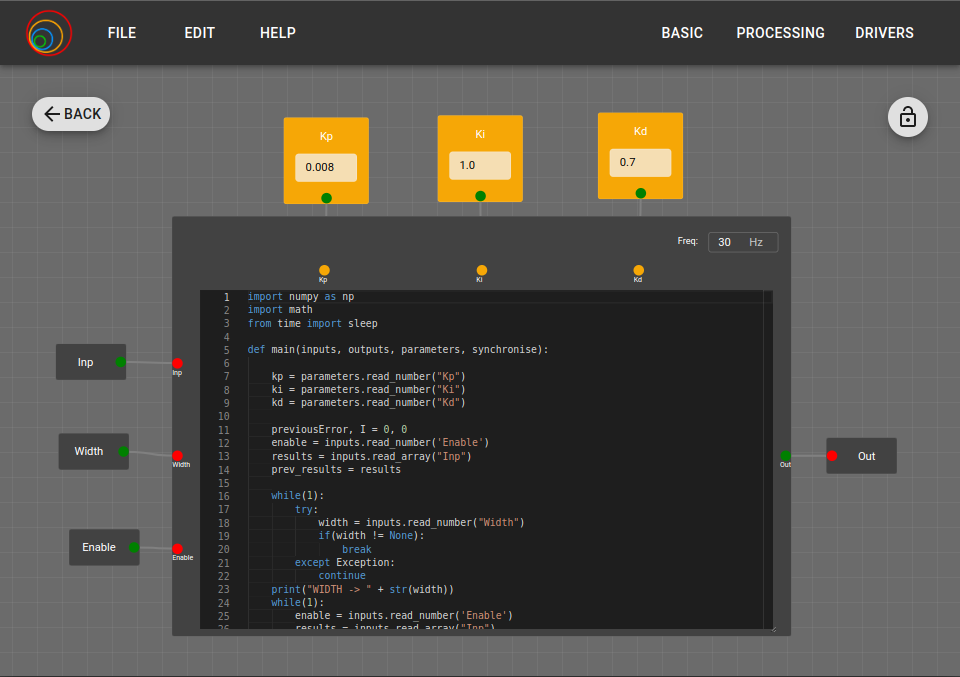
\includegraphics[width=10cm]{figs/c5/PID_follow_person.png}
    \end{center}
    \caption[Circuito del bloque PID sigue-persona]{Circuito del bloque PID del sigue-persona en VisualCircuit.}
    \label{fig:PID_follow_person}
\end{figure}

Analizando el código del bloque PID (\ref{cod:PID_follow_person}), se puede ver que primero lee los tres parámetros del controlador y entra en el
mismo bucle que se ha mencionado en el código bloque de decisión (\ref{cod:decision_follow_person}), donde se espera hasta obtener datos para
empezar a trabajar. Después, en el bucle principal sólo se analizan y envían los datos del PID en caso de que el bloque haya sido activado.\\

\begin{code}[H]
    \begin{lstlisting}[language=python]
        def main(inputs, outputs, parameters, synchronise):
            kp = parameters.read_number("Kp")
            ki = parameters.read_number("Ki")
            kd = parameters.read_number("Kd")
            previousError = 0
            I = 0
            max_rotation = 1
            enable = inputs.read_number('Enable')
            results = inputs.read_array("Inp")
            prev_results = results

            while(1):
                try:
                    width = inputs.read_number("Width")
                    if(width != None):
                        break
                except Exception:
                    continue
            while(1):
                enable = inputs.read_number('Enable')
                results = inputs.read_array("Inp")
                if(enable != 0):
                    if(enable == 1):
                        error = float(results[0]+results[2]/2) - width/2
                        prev_results = results
                    P = error
                    D = float(error) - float(previousError)
                    PIDvalue = (kp*P)  + (kd*D)
                    previousError = float(error)

                    angular_velocity = -PIDvalue
                    if(angular_velocity > max_rotation or angular_velocity < -max_rotation):
                        angular_velocity = max_rotation*angular_velocity/abs(angular_velocity)
                    data = [0,0,0,0,0, angular_velocity]
                    outputs.share_array("Out", data)
    \end{lstlisting}
    \caption[Código bloque PID sigue-persona]{Código del bloque del PID sigue-persona.}
    \label{cod:PID_follow_person}
\end{code}

\newpage

Como podemos ver en el código anterior (código \ref{cod:PID_follow_person}), el controlador usado finalmente es únicamente PD (sin parte integral).
La parte proporcional se consigue mediante la resta del resultado actual y el resultado objetivo, en este caso se trata del centro de la imagen,
por lo que se usa la mitad del ancho de la imagen.
Para la parte derivativa, se busca reducir los cambios bruscos, por lo que se resta el error actual con el error de la iteración anterior.\\

Una vez obtenida la velocidad angular, se manda al bloque de los motores. Este bloque es similar al creado en el apartado
\ref{sec:blocks_sensores} pero ahora con cuatro \textit{inputs}: \textit{Enable}, vel1 (rotación), vel2 (PID) y decisión.
En el código del bloque también se ha modificado la función \textit{main} para que lea las velocidades correspondientes al comportamiento actual y
que esta sea la velocidad que se comanda a los motores del robot.\\

\begin{code}[H]
    \begin{lstlisting}[language=python]
    while auto_enable:
        try:
            decision = inputs.read_number("Decision")
            if(decision == 0):
                velocities = inputs.read_array('Vels1')
            else:
                velocities = inputs.read_array('Vels2')
        except Exception:
            continue
\end{lstlisting}
\caption[Código bloque MotorDriver sigue-persona]{Código del bloque del \textit{MotorDriver} sigue-persona.}
\label{cod:MotorDriver_FP}
\end{code}

\subsection{Validación experimental}
\label{subsec:FP1_val}

Al probarlo todo junto usando el TurtleBot2 real, se puede observar que mientras la persona está quieta, la cámara la mantiene centrada y,
cuando empieza a moverse hacia un lado, el robot gira para volver a ponerlo en el centro de la imagen, obteniendo el resultado esperado.\\

En la siguiente secuencia de imágenes se puede observar el movimiento que ha seguido el robot tras la ejecución:

\begin{figure} [H]
    \begin{center}
        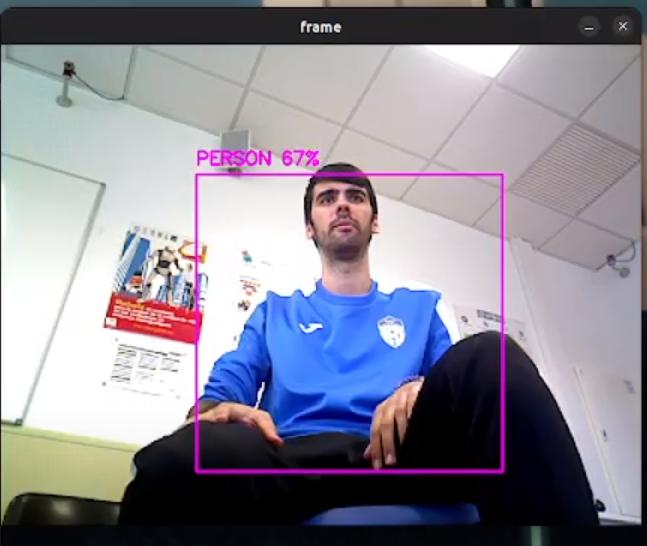
\includegraphics[width=7cm]{figs/c5/sec_rot1.png}
        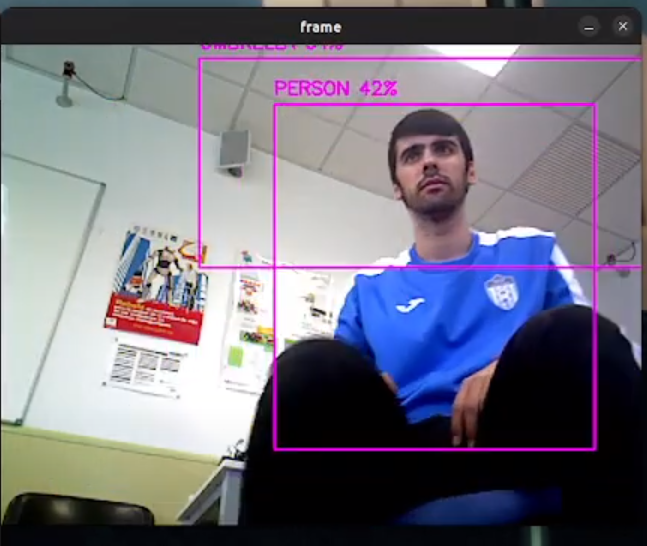
\includegraphics[width=7cm]{figs/c5/sec_rot2.png}
        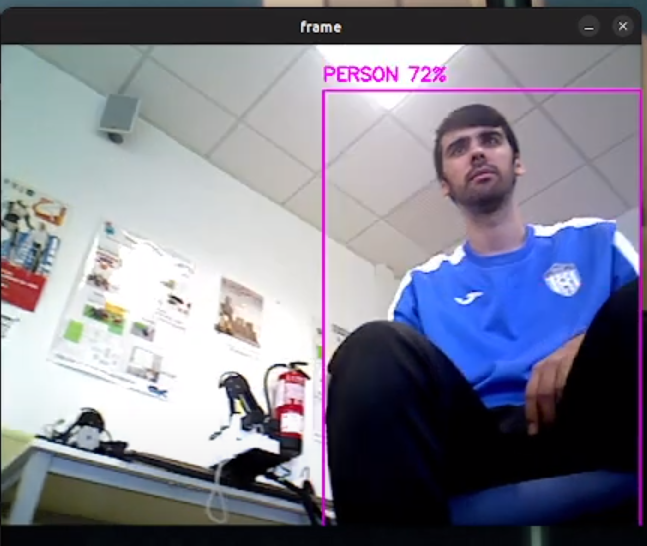
\includegraphics[width=7cm]{figs/c5/sec_rot3.png}
        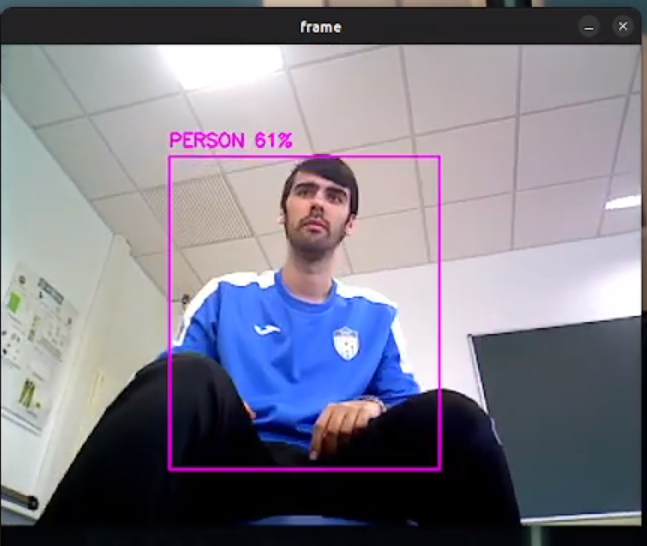
\includegraphics[width=7cm]{figs/c5/sec_rot4.png}
    \end{center}
    \caption[Secuencia sigue-personas rotación]{Secuencia de imágenes del sigue-personas sólo con rotación. Imagenes obtenidas de Youtube\footnotemark.}
    \label{fig:sec_FP_rot}
\end{figure}
\footnotetext{\textbf{Vídeo}: \url{https://www.youtube.com/watch?v=Uir_iqMOplc&ab_channel=Tapii}}

\section{Seguimiento completo de persona}
\label{sec:FP_2}

\subsection{Diseño del comportamiento}
\label{subsec:FP2_dis_comp}

La segunda etapa combina el comportamiento anterior con seguir linealmente a la persona. Para ello se debe leer también la información
sobre la profundidad que nos da la cámara.\\

Como podemos ver, toda la rama inferior de bloques es la que se encarga del movimiento lineal, obteniendo la distancia con la persona mediante
la profundidad captada por la cámara y buscando que el robot se mantenga a una distancia constante de la persona mediante el bloque PID.
Por otro lado, la rama superior se encarga del movimiento angular.

\begin{figure} [H]
    \begin{center}
        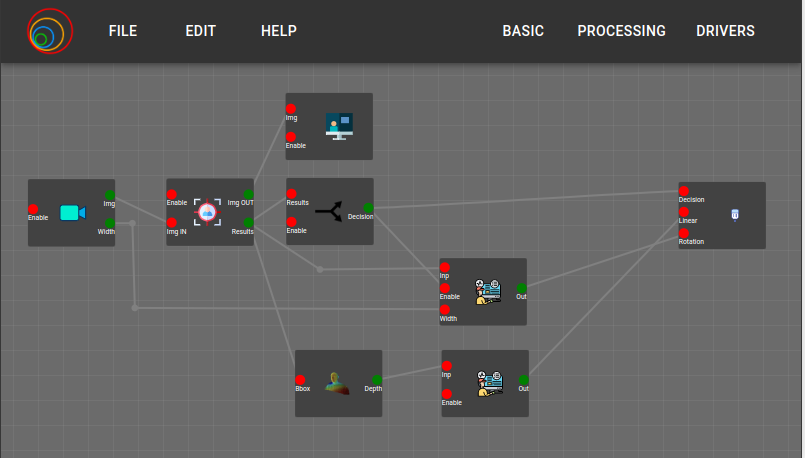
\includegraphics[width=12cm]{figs/c5/follow_person_final_model.png}
    \end{center}
    \caption[Circuito sigue-personas inicial]{Circuito inicial del algoritmo sigue-persona.}
    \label{fig:final_follow_person}
\end{figure}

\subsection{Bloques específicos de la lógica de esta aplicación}
\label{subsec:FP2_blocks}

La única parte de esta rama que ha cambiado frente a la anterior etapa es que en ésta no existe un bloque que envíe la velocidad de rotación, sino que está
directamente implementado en el bloque MotorDriverROS2 y, dependiendo de la decisión, se envía la rotación estática o se envían
las velocidades de los bloques PID.

\begin{code}[H]
    \begin{lstlisting}[language=python]
        while auto_enable:
            try:
                decision = inputs.read_number("Decision")
                if(decision == 0):
                    velocities = [0,0,0,0,0,0.05]
                else:
                    velocities = inputs.read_array('Vels2')
                    velocities[0] = inputs.read_number('Linear')
            except Exception:
                continue

    \end{lstlisting}
    \caption[Código bloque MotorDriver sigue-persona modificado]{Código del bloque del \textit{MotorDriver} sigue-persona modificado.}
    \label{cod:MotorDriver_FP_final}
\end{code}

En cuanto a la rama inferior, el bloque principal es el que recibe la información de la profundidad. Esta información viene en forma
de \textit{PointCloud2} (\textit{sensor\_msgs/msg/PointCloud2}) que, como  podemos ver en la imagen \ref{fig:PC2_struct}, envía los datos del sensor en el
campo \textit{data}, por lo que esto será lo que guardemos en la variable global del bloque del sensor y será lo que enviemos por el cable.\\

\begin{figure} [H]
    \begin{center}
        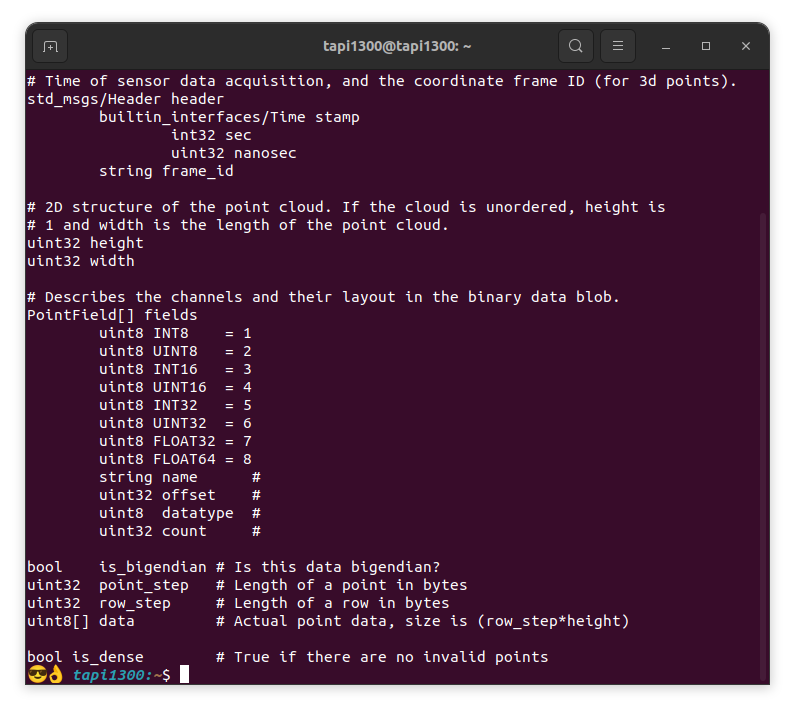
\includegraphics[width=10cm]{figs/c5/PointCloud2_data.png}
    \end{center}
    \caption[Estructura mensaje PointCloud2]{Estructura del tipo de mensaje \textit{sensor\_msgs/msg/PointCloud2.}}
    \label{fig:PC2_struct}
\end{figure}

La forma en la que se guardan los datos dentro del campo \textit{data} es en bytes, siguiendo la siguiente estructura para cada punto de la cámara (640x480 = 307200 puntos):
12 bytes para x,y,z (4 bytes cada coordenada), 4 bytes vacíos, 4 bytes para el color del punto y otros 12 bytes vacíos. Esto hace que en el \textit{array} de datos
aparezcan 9830400 valores y la búsqueda final sea el número de filas (coordenada Y) multiplicado por el ancho total de la imagen más la posición actual de la coordenada X
multiplicado por 32 (posiciones que ocupa cada pixel en el array) y sumamos 8 para obtener la posición inicial de la coordenada Z (\textit{(width*y+x)*32+8}). Luego, usando la función
``\textit{unpack}" del paquete \textit{struct} se transforman los siguiente 4 bytes (correspondientes a la coordenada Z) a un \textit{float} y se obteniene
la distancia entre el robot y el centro de la \textit{BoundingBox} de la persona.

\begin{code}[H]
    \begin{lstlisting}[language=python]
    # IMPORT
    from sensor_msgs.msg import PointCloud2
    from struct import unpack

    # CALLBACK DENTRO DE LA CLASE
        def callback(self, msg):
            global measure
            measure = msg.data

    # BUCLE DENTRO DEL MAIN
        while(1):
            bbox = inputs.read_array("Bbox")
            if bbox is None:
                continue
            try:
                x = int(bbox[0]+bbox[2]/2)
                y = int(bbox[1]+bbox[3]/2)
            except:
                continue

            rclpy.spin_once(depth_subscriber)
            point = (width*y+x)*32+8
            depth = unpack('f', measure[point:point+4])
            outputs.share_array("Depth",depth)   
            synchronise()
    \end{lstlisting}
    \caption[Código bloque Camera-Depth sigue-persona]{Código del bloque del \textit{PointCloud2} del sigue-persona.}
    \label{cod:PC2_block_FP}
\end{code}

Esta información llega a un segundo bloque PID, que es el que se encarga de mantener esta distancia con la persona en 1.5 metros. El código de este bloque
es similar al del otro bloque PID (\ref{cod:PID_follow_person}), pero ahora no se necesita una velocidad límite (el mínimo y máximo posibles linealmente
no son tan peligrosos en comparación a las velocidades angulares altas).

\begin{code}[H]
    \begin{lstlisting}[language=python]
        import numpy as np
        import math
        from time import sleep
        def main(inputs, outputs, parameters, synchronise):
            auto_enable = True
            try:
                enable = inputs.read_number("Enable")
            except Exception:
                auto_enable = True
            kp = parameters.read_number("Kp")
            ki = parameters.read_number("Ki")
            kd = parameters.read_number("Kd")
            previousError, I = 0, 0
    \end{lstlisting}
\end{code}
\begin{code}[H]
    \begin{lstlisting}[language=python]
            while(auto_enable or inputs.read_number('Enable')):
                msg = inputs.read_number("Inp")
                if msg is None:
                    continue
                error = float(msg) - 1.5
                sleep(0.01)
        
                P = error
                D = error - previousError
                PIDvalue = (kp*P) + (kd*D)
                previousError = error
    
                linear_velocity = PIDvalue
                if msg == 0:
                    linear_velocity = 0
                outputs.share_number("Out", linear_velocity)
                synchronise()
    \end{lstlisting}
    \caption[Código bloque PID lineal sigue-persona]{Código del bloque del PID de velocidad lineal del sigue-persona.}
    \label{cod:PID_linear_FP}
\end{code}

\subsection{Validación experimental}
\label{subsec:FP2_val}

Para comprobar que la aplicación sigue-personas completa funcionase, se puso al robot dentro de la sala del laboratorio y se grabó cómo seguía a una persona
desde dos ángulos: la visión del robot y la visión de la persona (para observar qué movimientos hizo el robot). Los resultados que se pueden observar en la siguiente
secuencia de imágenes (figura \ref{fig:sec_FP_final}) extraídas del vídeo oficial demuestran el correcto funcionamiento de la aplicación y de los bloques desarrollados.\\



\begin{figure} [H]
    \begin{center}
        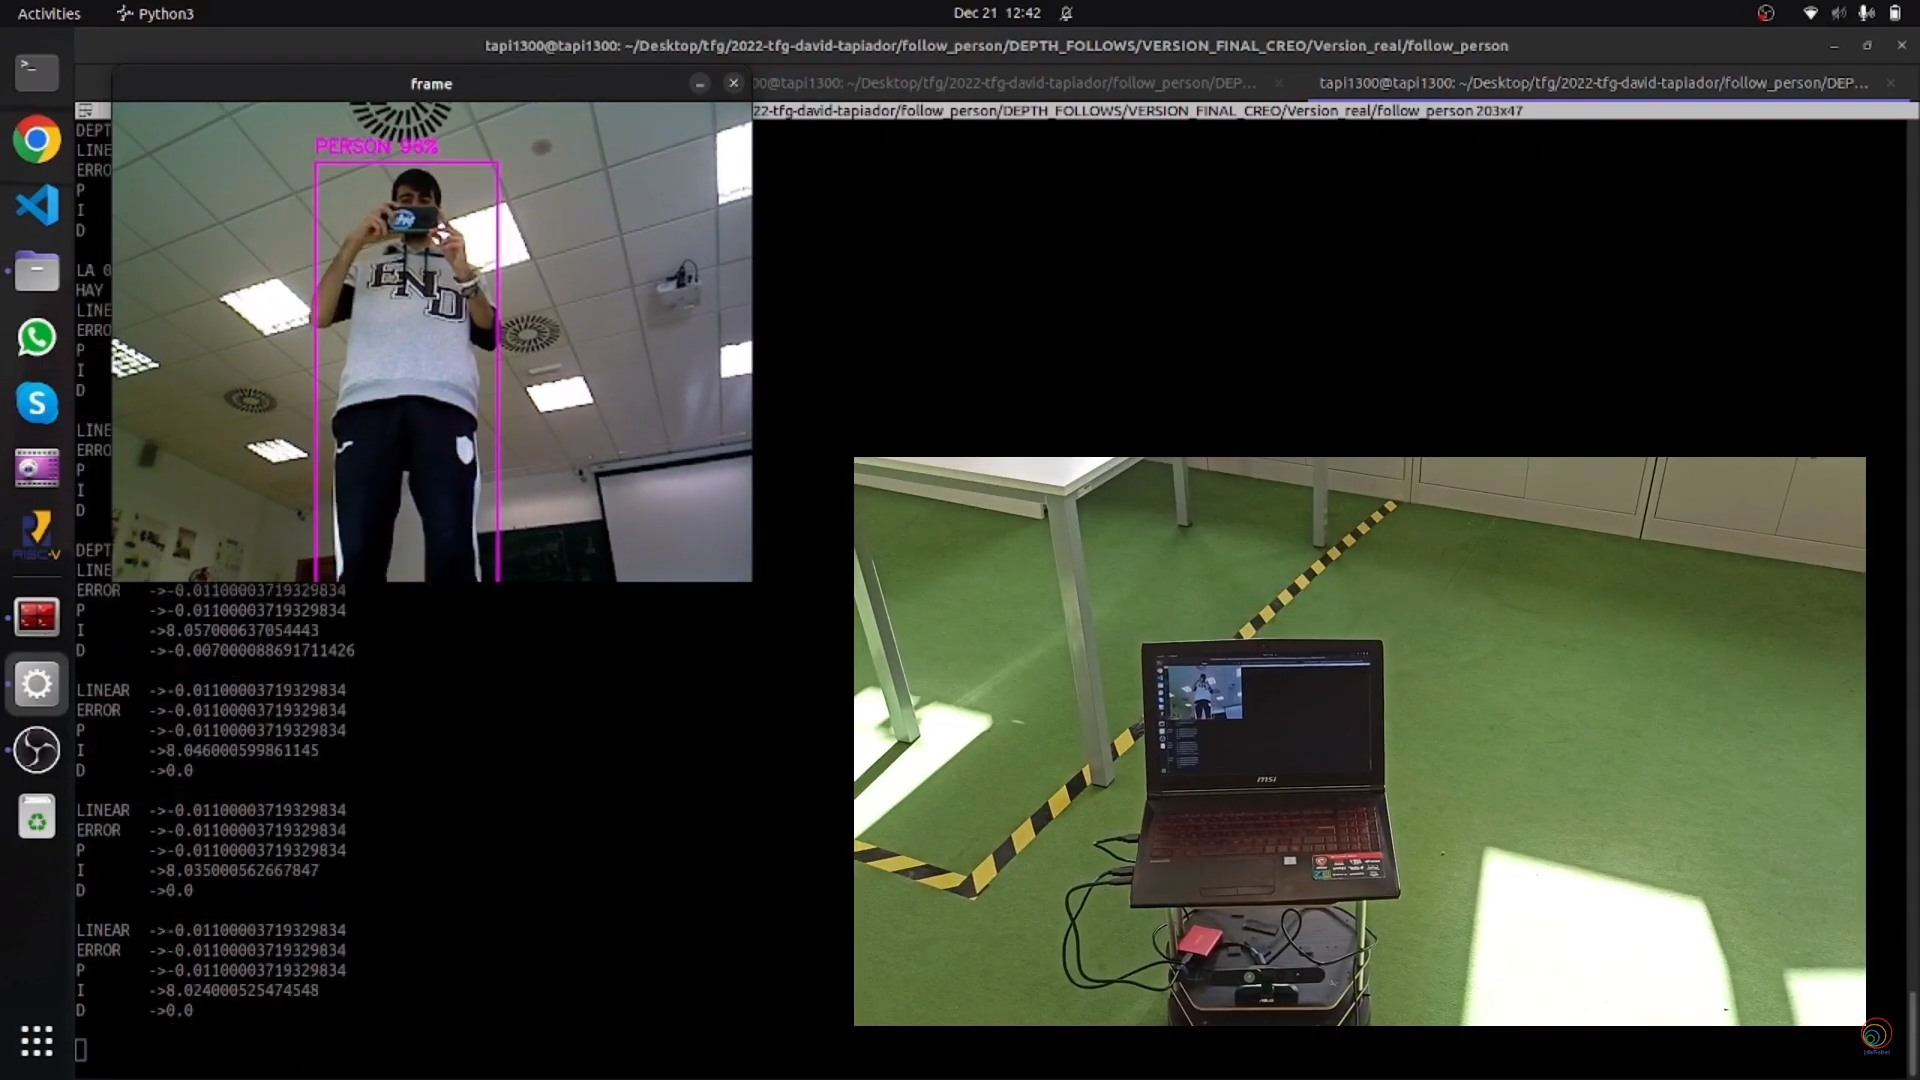
\includegraphics[width=7cm]{figs/c5/fp_final1.png}
        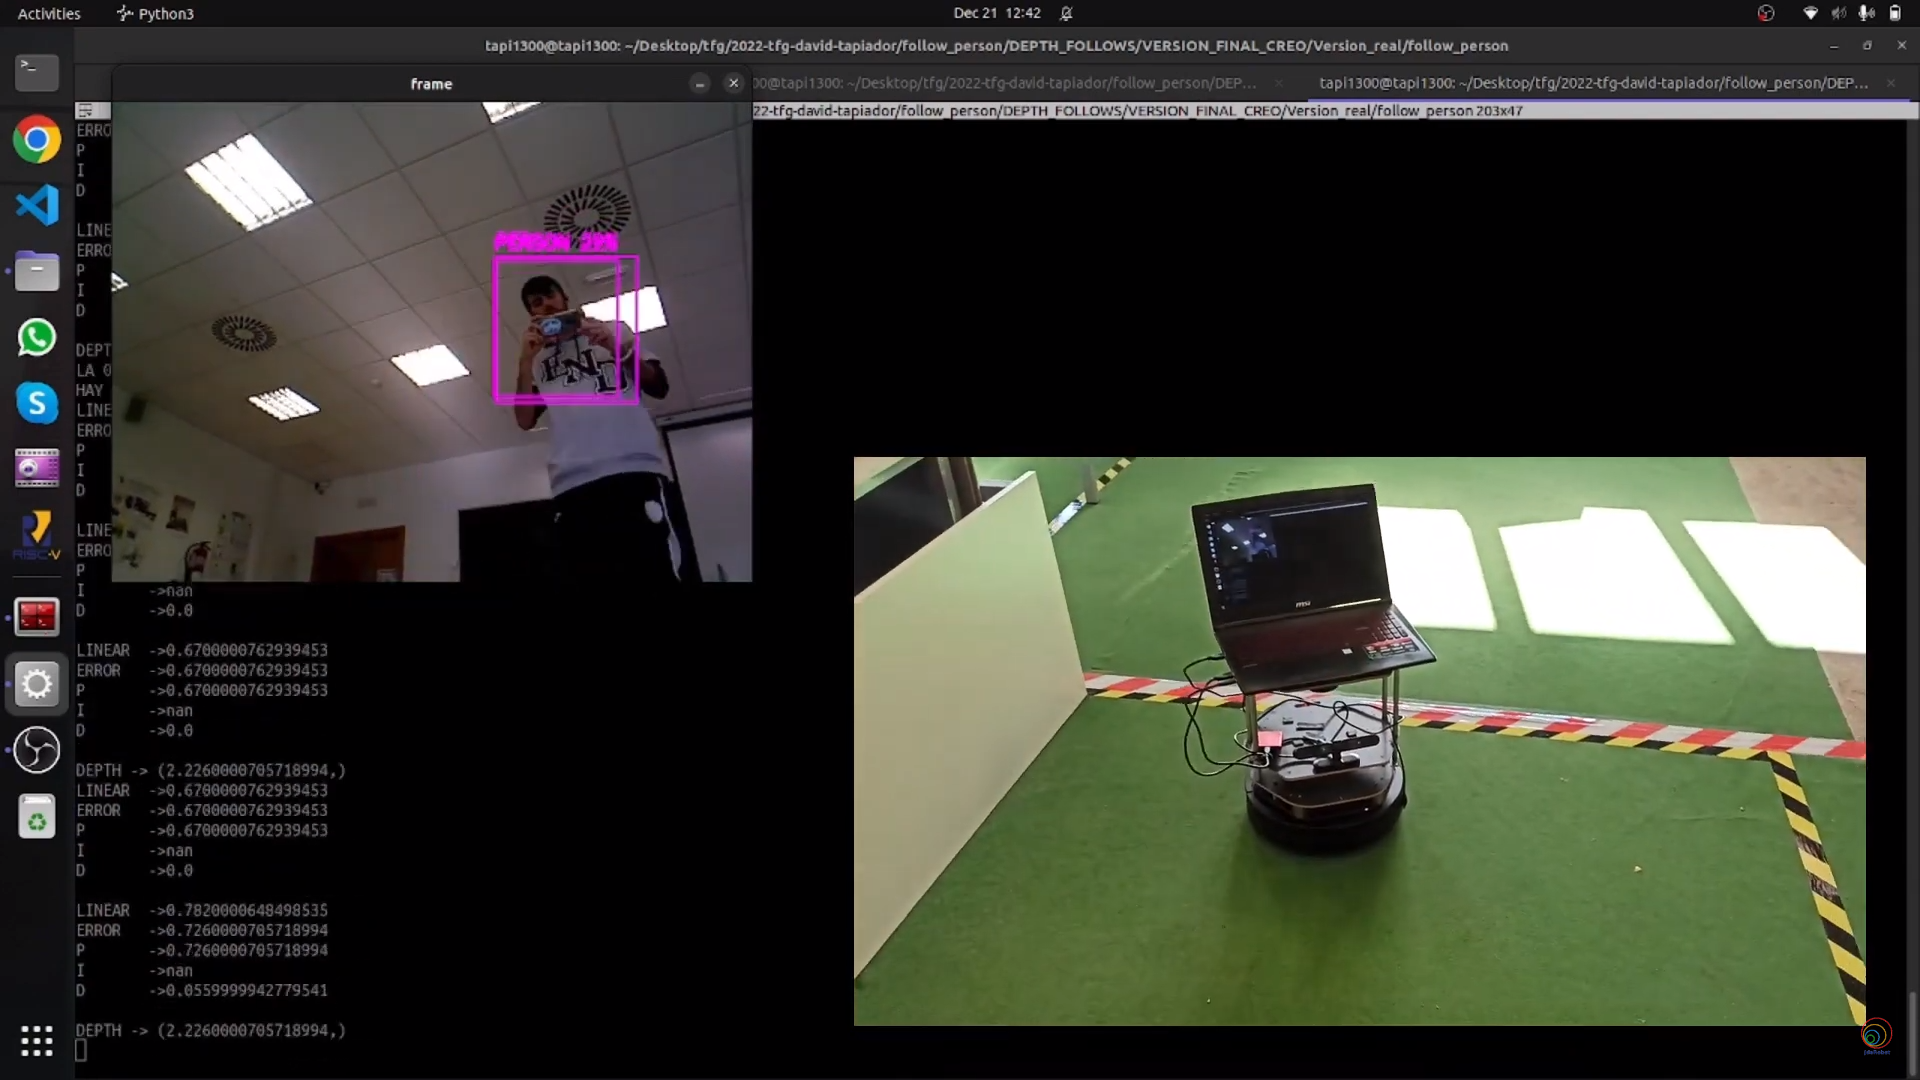
\includegraphics[width=7cm]{figs/c5/fp_final2.png}
    \end{center}
\end{figure}
\begin{figure} [H]
    \begin{center}
        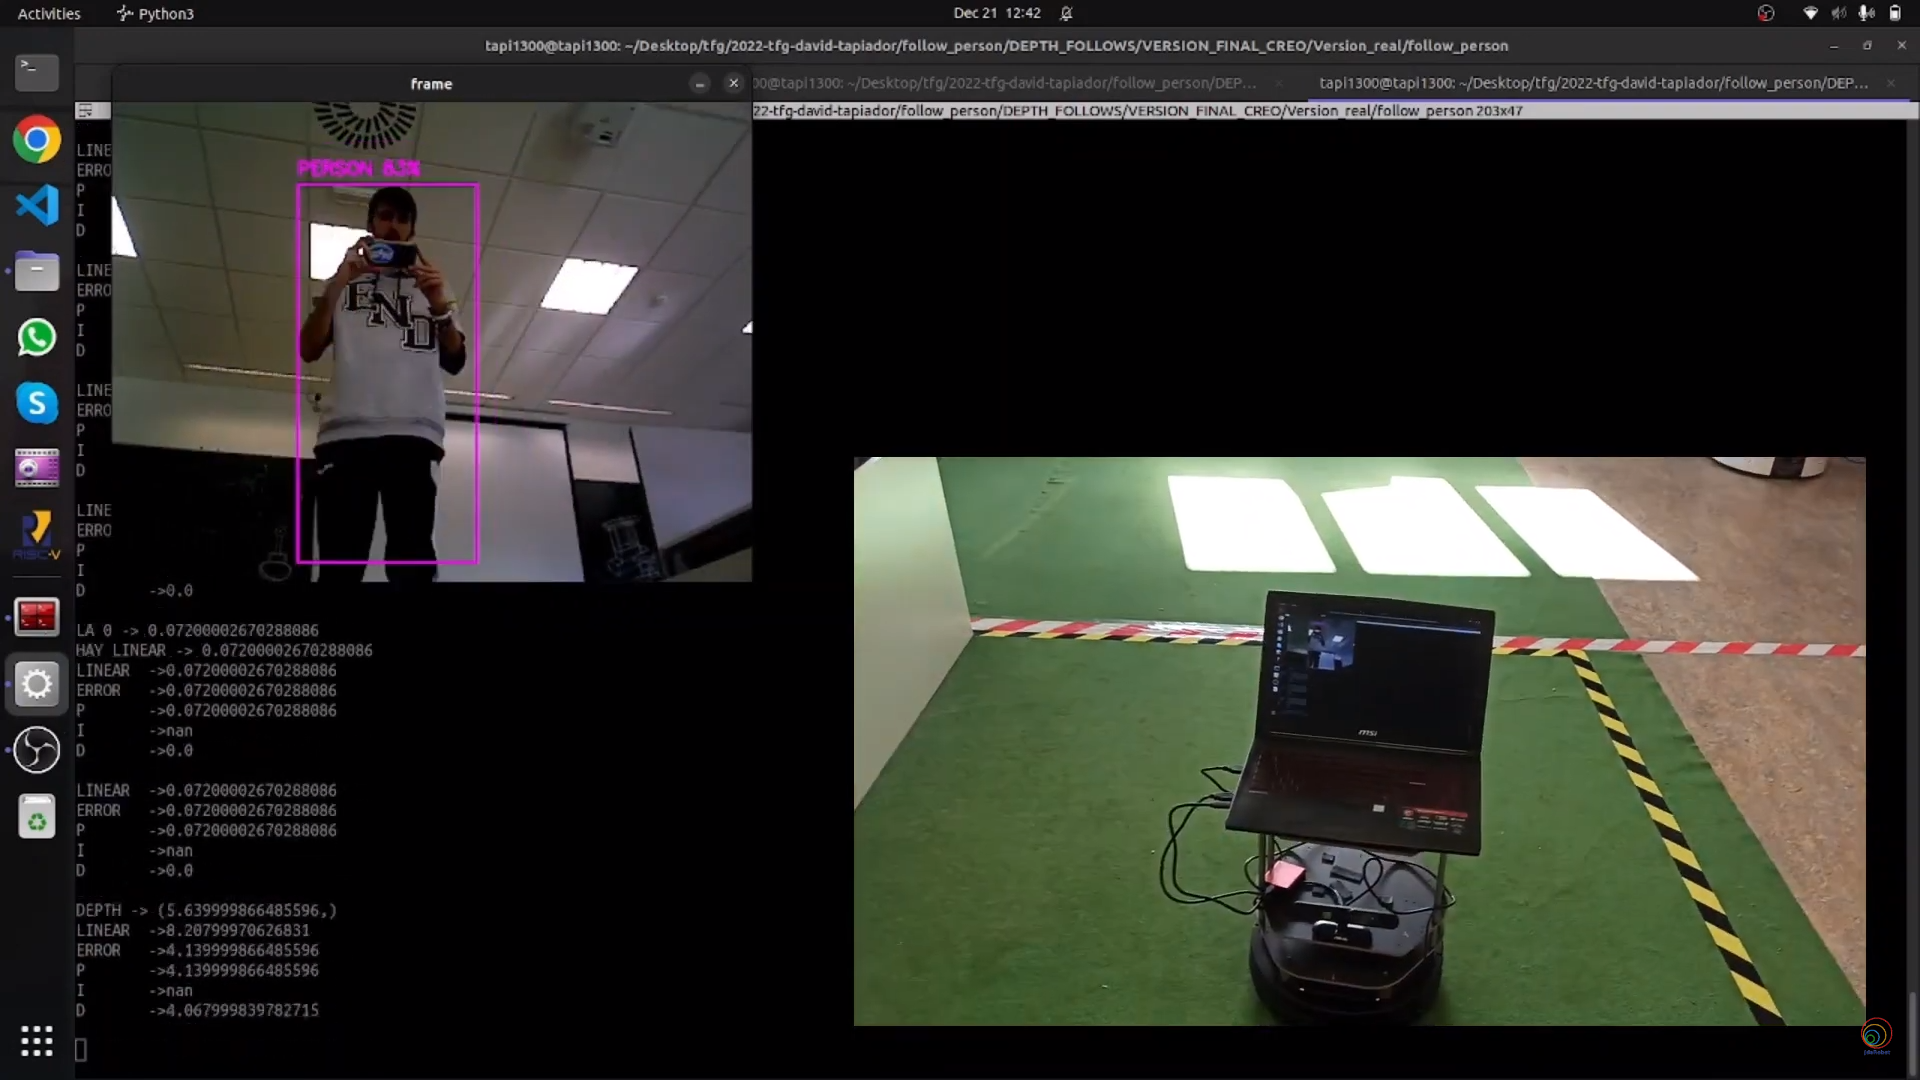
\includegraphics[width=7cm]{figs/c5/fp_final3.png}
        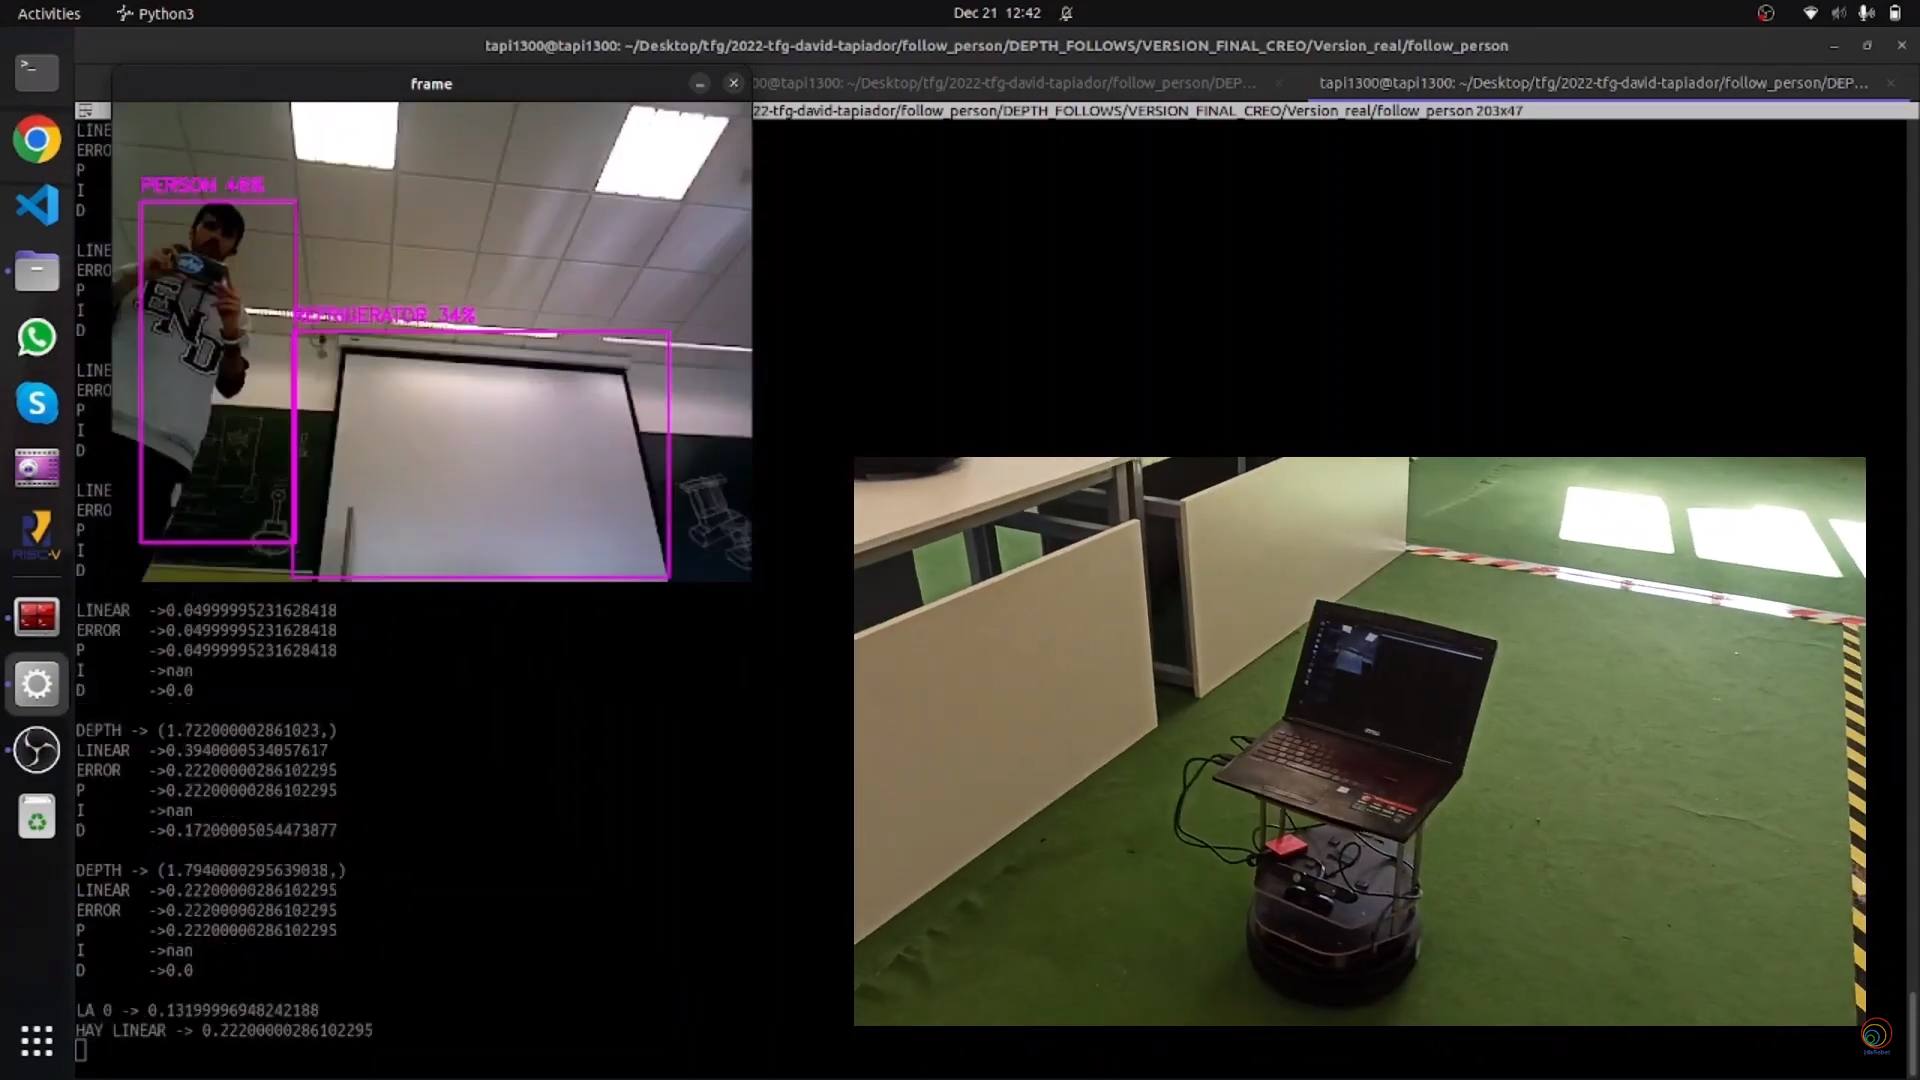
\includegraphics[width=7cm]{figs/c5/fp_final4.png}
    \end{center}
    \caption[Secuencia sigue-personas completo resultado final]{Secuencia de imágenes del sigue-personas completo. Imagenes obtenidas de Youtube\footnotemark.}
    \label{fig:sec_FP_final}
\end{figure}
\footnotetext{\textbf{Vídeo}: \url{https://www.youtube.com/watch?v=IknpvAs_jAo&ab_channel=JdeRobot}}




